% !TEX TS-program = pdflatex
% !TEX encoding = UTF-8 Unicode

% This is a simple template for a LaTeX document using the "article" class.
% See "book", "report", "letter" for other types of document.

\documentclass[20pt]{article} % use larger type; default would be 10pt

\usepackage[utf8]{inputenc} % set input encoding (not needed with XeLaTeX)

%%% Examples of Article customizations
% These packages are optional, depending whether you want the features they provide.
% See the LaTeX Companion or other references for full information.

%%% PAGE DIMENSIONS
\usepackage{geometry} % to change the page dimensions
\geometry{a4paper} % or letterpaper (US) or a5paper or....
% \geometry{margin=2in} % for example, change the margins to 2 inches all round
% \geometry{landscape} % set up the page for landscape
%   read geometry.pdf for detailed page layout information

\usepackage{graphicx} % support the \includegraphics command and options

% \usepackage[parfill]{parskip} % Activate to begin paragraphs with an empty line rather than an indent

%%% PACKAGES
\usepackage{booktabs} % for much better looking tables
\usepackage{array} % for better arrays (eg matrices) in maths
\usepackage{paralist} % very flexible & customisable lists (eg. enumerate/itemize, etc.)
\usepackage{verbatim} % adds environment for commenting out blocks of text & for better verbatim
%\usepackage{subfig} % make it possible to include more than one captioned figure/table in a single float
\usepackage{mathtools}
\usepackage{graphicx} % supports images in latex
% These packages are all incorporated in the memoir class to one degree or another...

\usepackage{graphicx}
\usepackage{subcaption}

%%% Other stuff
\DeclarePairedDelimiter\ceil{\lceil}{\rceil}
\DeclarePairedDelimiter\floor{\lfloor}{\rfloor}

%%% HEADERS & FOOTERS
\usepackage{fancyhdr} % This should be set AFTER setting up the page geometry
\pagestyle{fancy} % options: empty , plain , fancy
\renewcommand{\headrulewidth}{0pt} % customise the layout...
\lhead{}\chead{}\rhead{}
\lfoot{}\cfoot{\thepage}\rfoot{}

%%% SECTION TITLE APPEARANCE
\usepackage{sectsty}
\allsectionsfont{\sffamily\mdseries\upshape} % (See the fntguide.pdf for font help)
% (This matches ConTeXt defaults)

%%% ToC (table of contents) APPEARANCE
\usepackage[nottoc,notlof,notlot]{tocbibind} % Put the bibliography in the ToC
\usepackage[titles,subfigure]{tocloft} % Alter the style of the Table of Contents
\renewcommand{\cftsecfont}{\rmfamily\mdseries\upshape}
\renewcommand{\cftsecpagefont}{\rmfamily\mdseries\upshape} % No bold!

%%% graphics path


%%% END Article customizations

%%% nice things to keep around
%\begin{figure}[!htbp]
%  	\centering
%   	\begin{subfigure}[p]{0.5\linewidth}
%    	\includegraphics[width=\linewidth]{}
%   	\end{subfigure}
%\end{figure} 

% \noindent\rule{2cm}{0.4pt} 
%%% puts a small horizontal line

% \mathcal{O} 
%%% big O notation

% \begin{table}[!htbp]
% \caption{Forward slash.}
% \[\begin{array}{c|ccccc} 
% abc/def & 1 & 2 & 3 & 4 & 5\\
% \hline
% 1 & a & b & c & d & e\\
% 2 & f & g & h & i & j\\
% 3 & k & l & m & n & o\\
% \end{array}\]
% \end{table}

%%% The "real" document content comes below...

\title{Formal Languages Homework 6}
\author{Liam Dillingham}
%\date{} % Activate to display a given date or no date (if empty),
         % otherwise the current date is printed 

\begin{document}
\maketitle

\section{Problem 6.1.1}
Suppose the PDA $\!P = (\{q, p\}, \{0,1\}, \{Z_0,X\}, \delta, q , Z_0, \{p\})$ has the following transition function
\begin{enumerate}
\item $\delta(q, 0, Z_0) = \{(q, XZ_0)\}$.
\item $\delta(q, 0, X) = \{(q, XX)\}$.
\item $\delta(q, 1, X) = \{(q, X)\}$.
\item $\delta(q, \epsilon, X) = \{(p, \epsilon)\}$.
\item $\delta(p, \epsilon, X) = \{(p, \epsilon)\}$.
\item $\delta(p, 1, X) = \{(p, XX)\}$.
\item $\delta(p, 1, Z_0) = \{(p, \epsilon)\}$.
\end{enumerate}
Starting from the initial ID $(q, w, Z_0)$, show all the reachable ID's when the input $w$ is:
\subsection{a). 01.}
\begin{figure}[!htbp]
  	\centering
   	\begin{subfigure}[p]{0.5\linewidth}
    	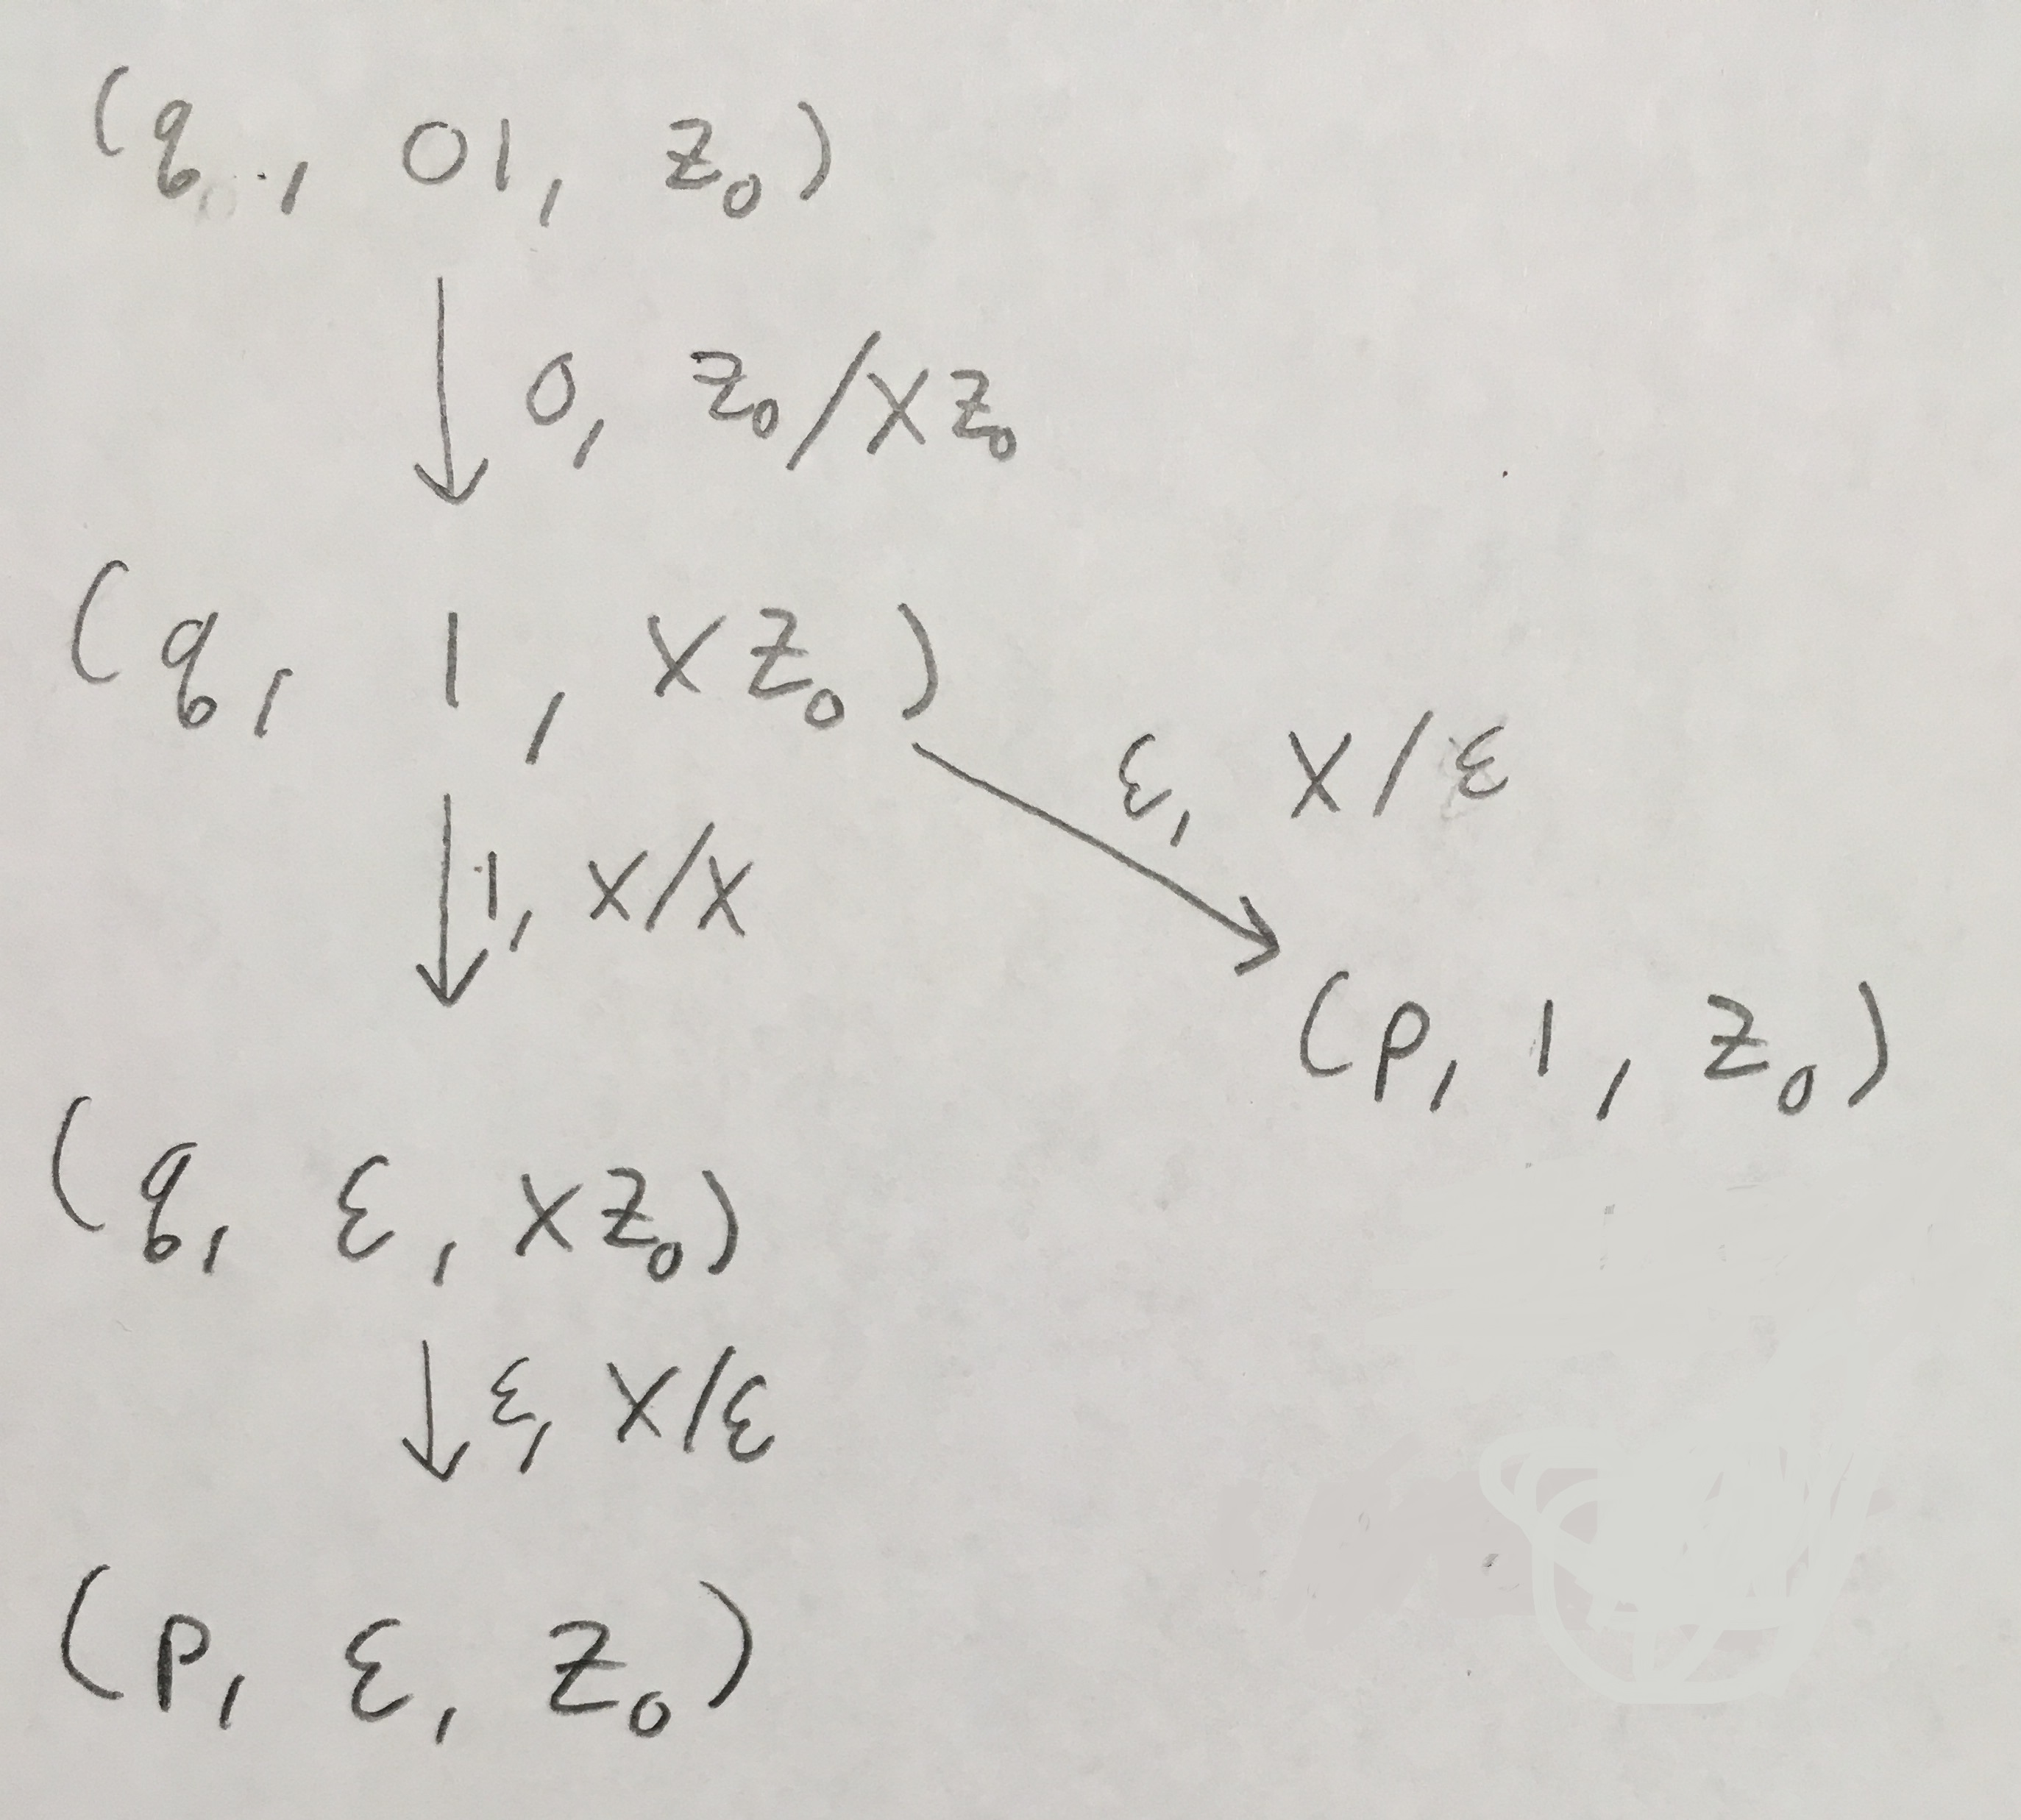
\includegraphics[width=\linewidth]{./figures/h7-1.jpg}
   	\end{subfigure}
\end{figure} 
\newpage
\subsection{b). 0011.}
\begin{figure}[!htbp]
  	\centering
   	\begin{subfigure}[p]{0.8\linewidth}
    	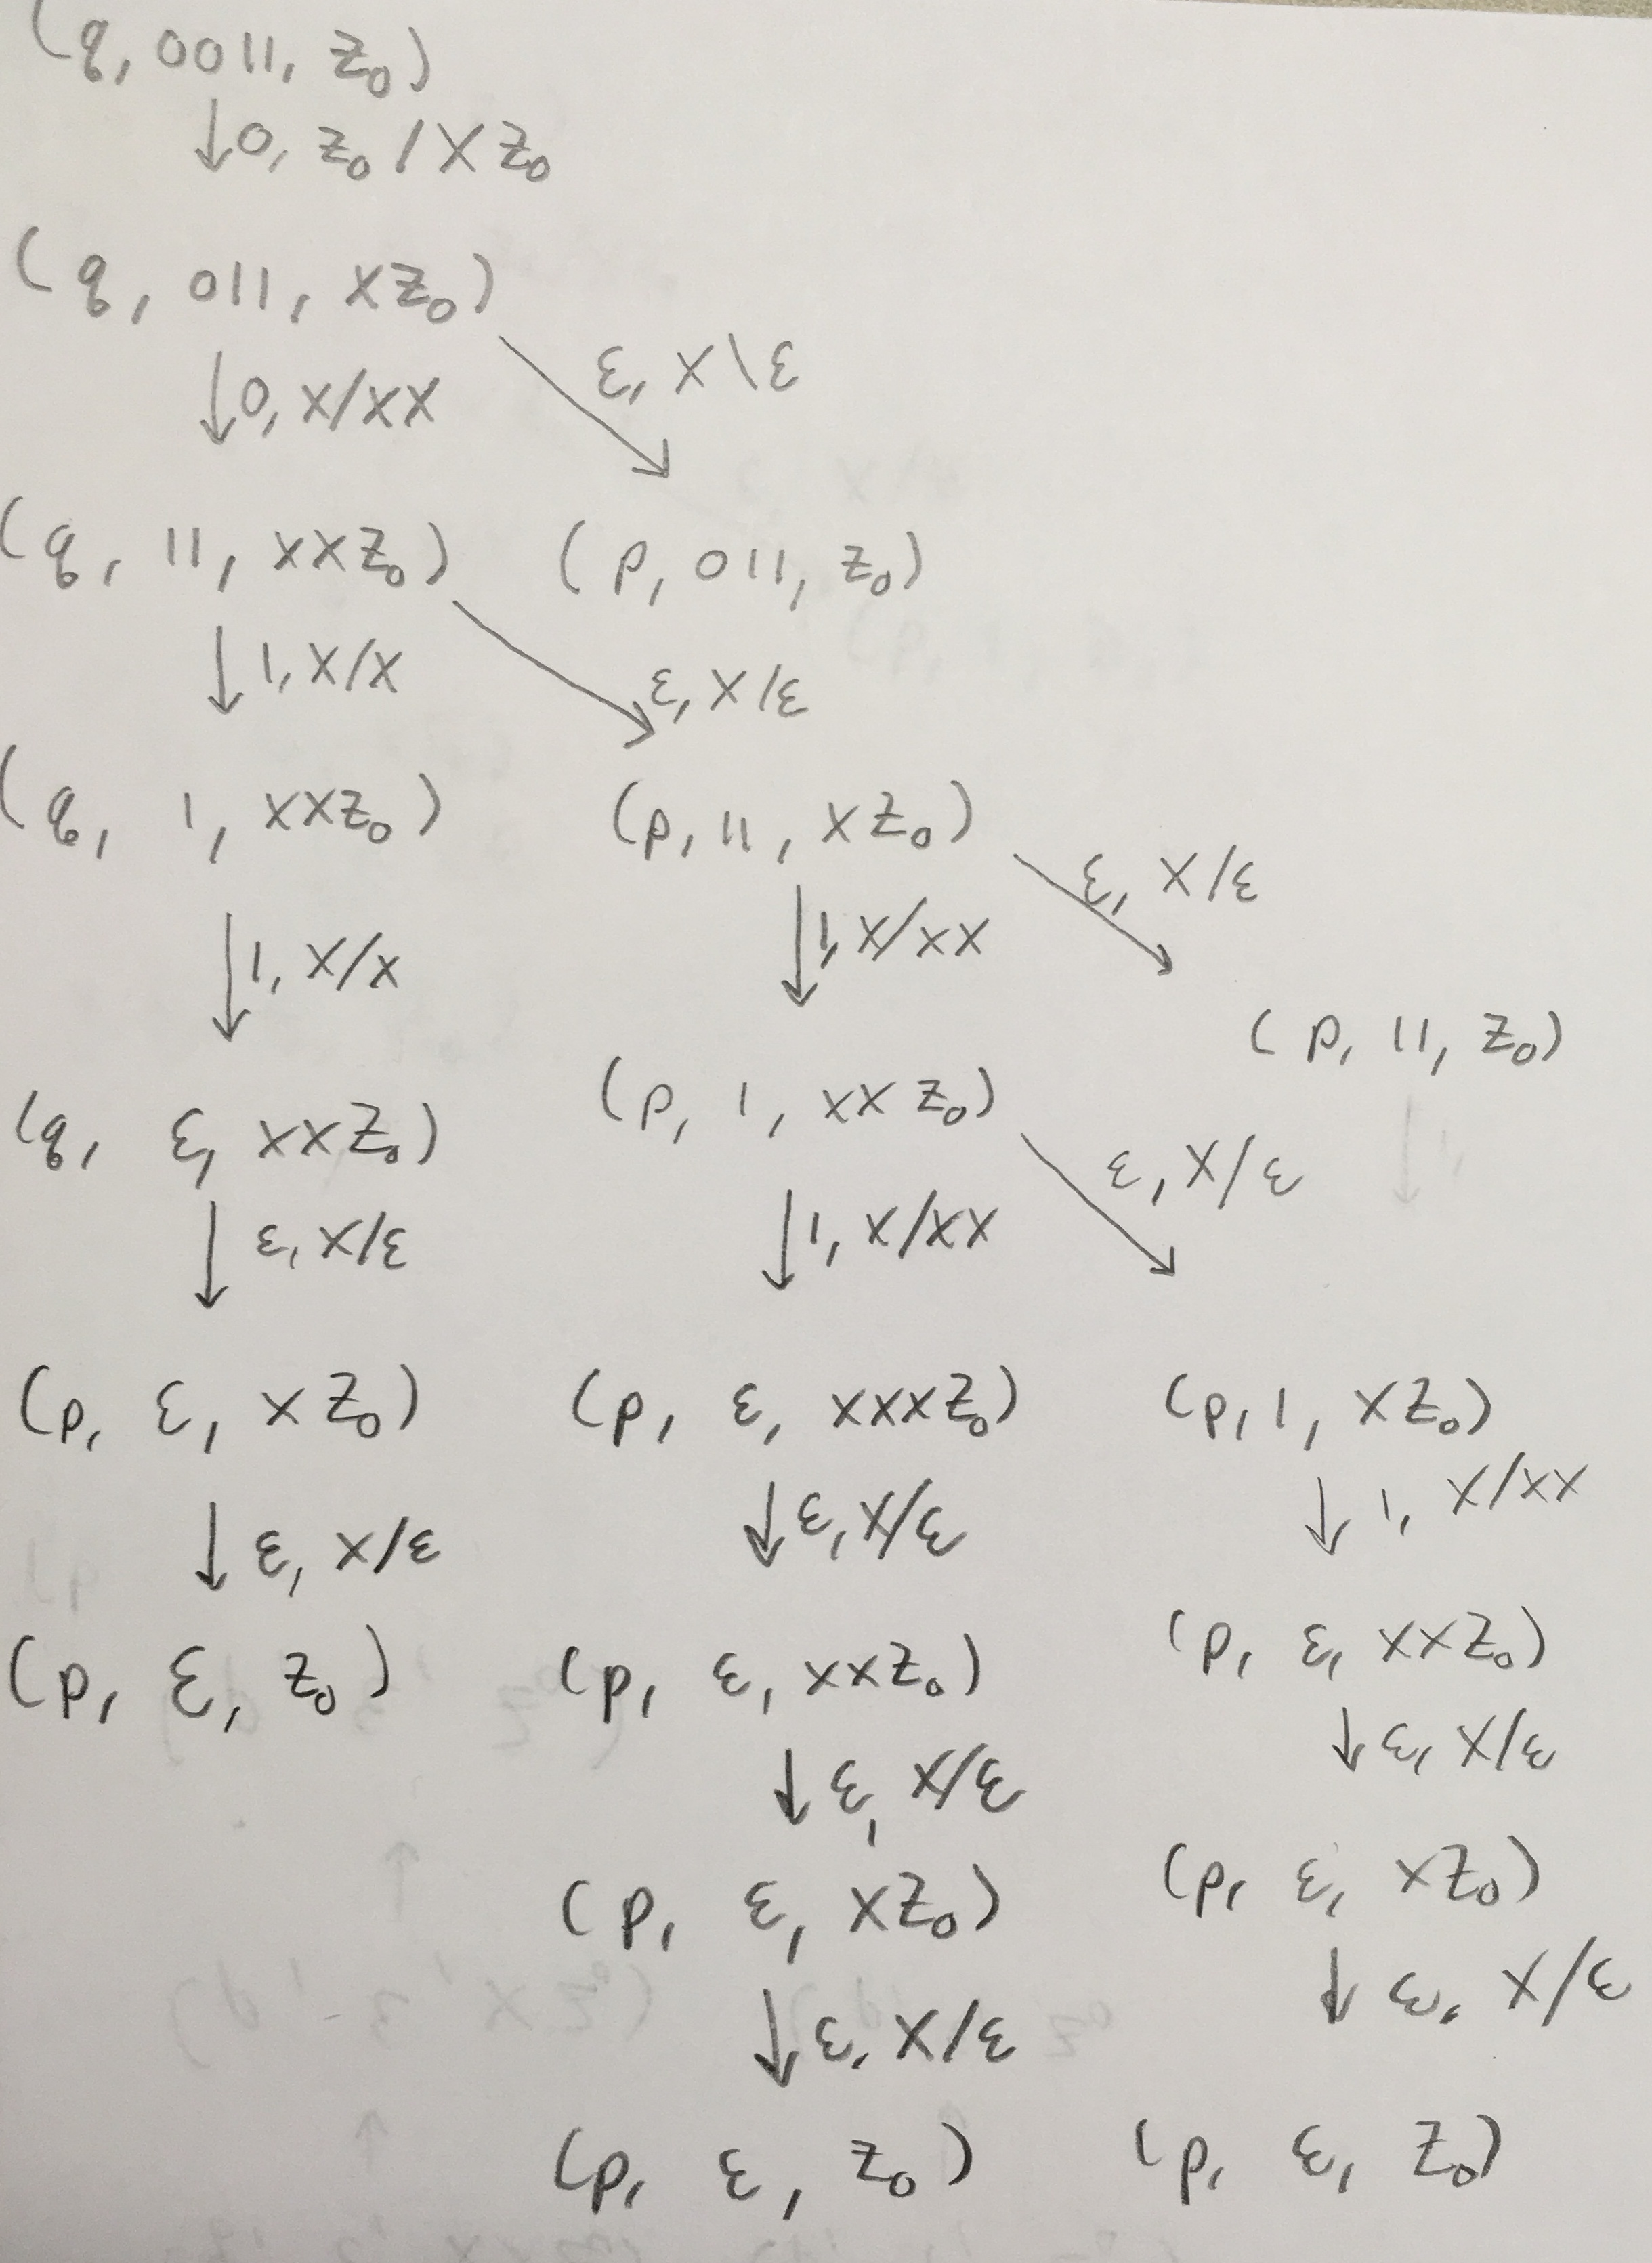
\includegraphics[width=\linewidth]{./figures/h7-2.jpg}
   	\end{subfigure}
\end{figure} 
\newpage
\subsection{c). 010.}
\begin{figure}[!htbp]
  	\centering
   	\begin{subfigure}[p]{0.6\linewidth}
    	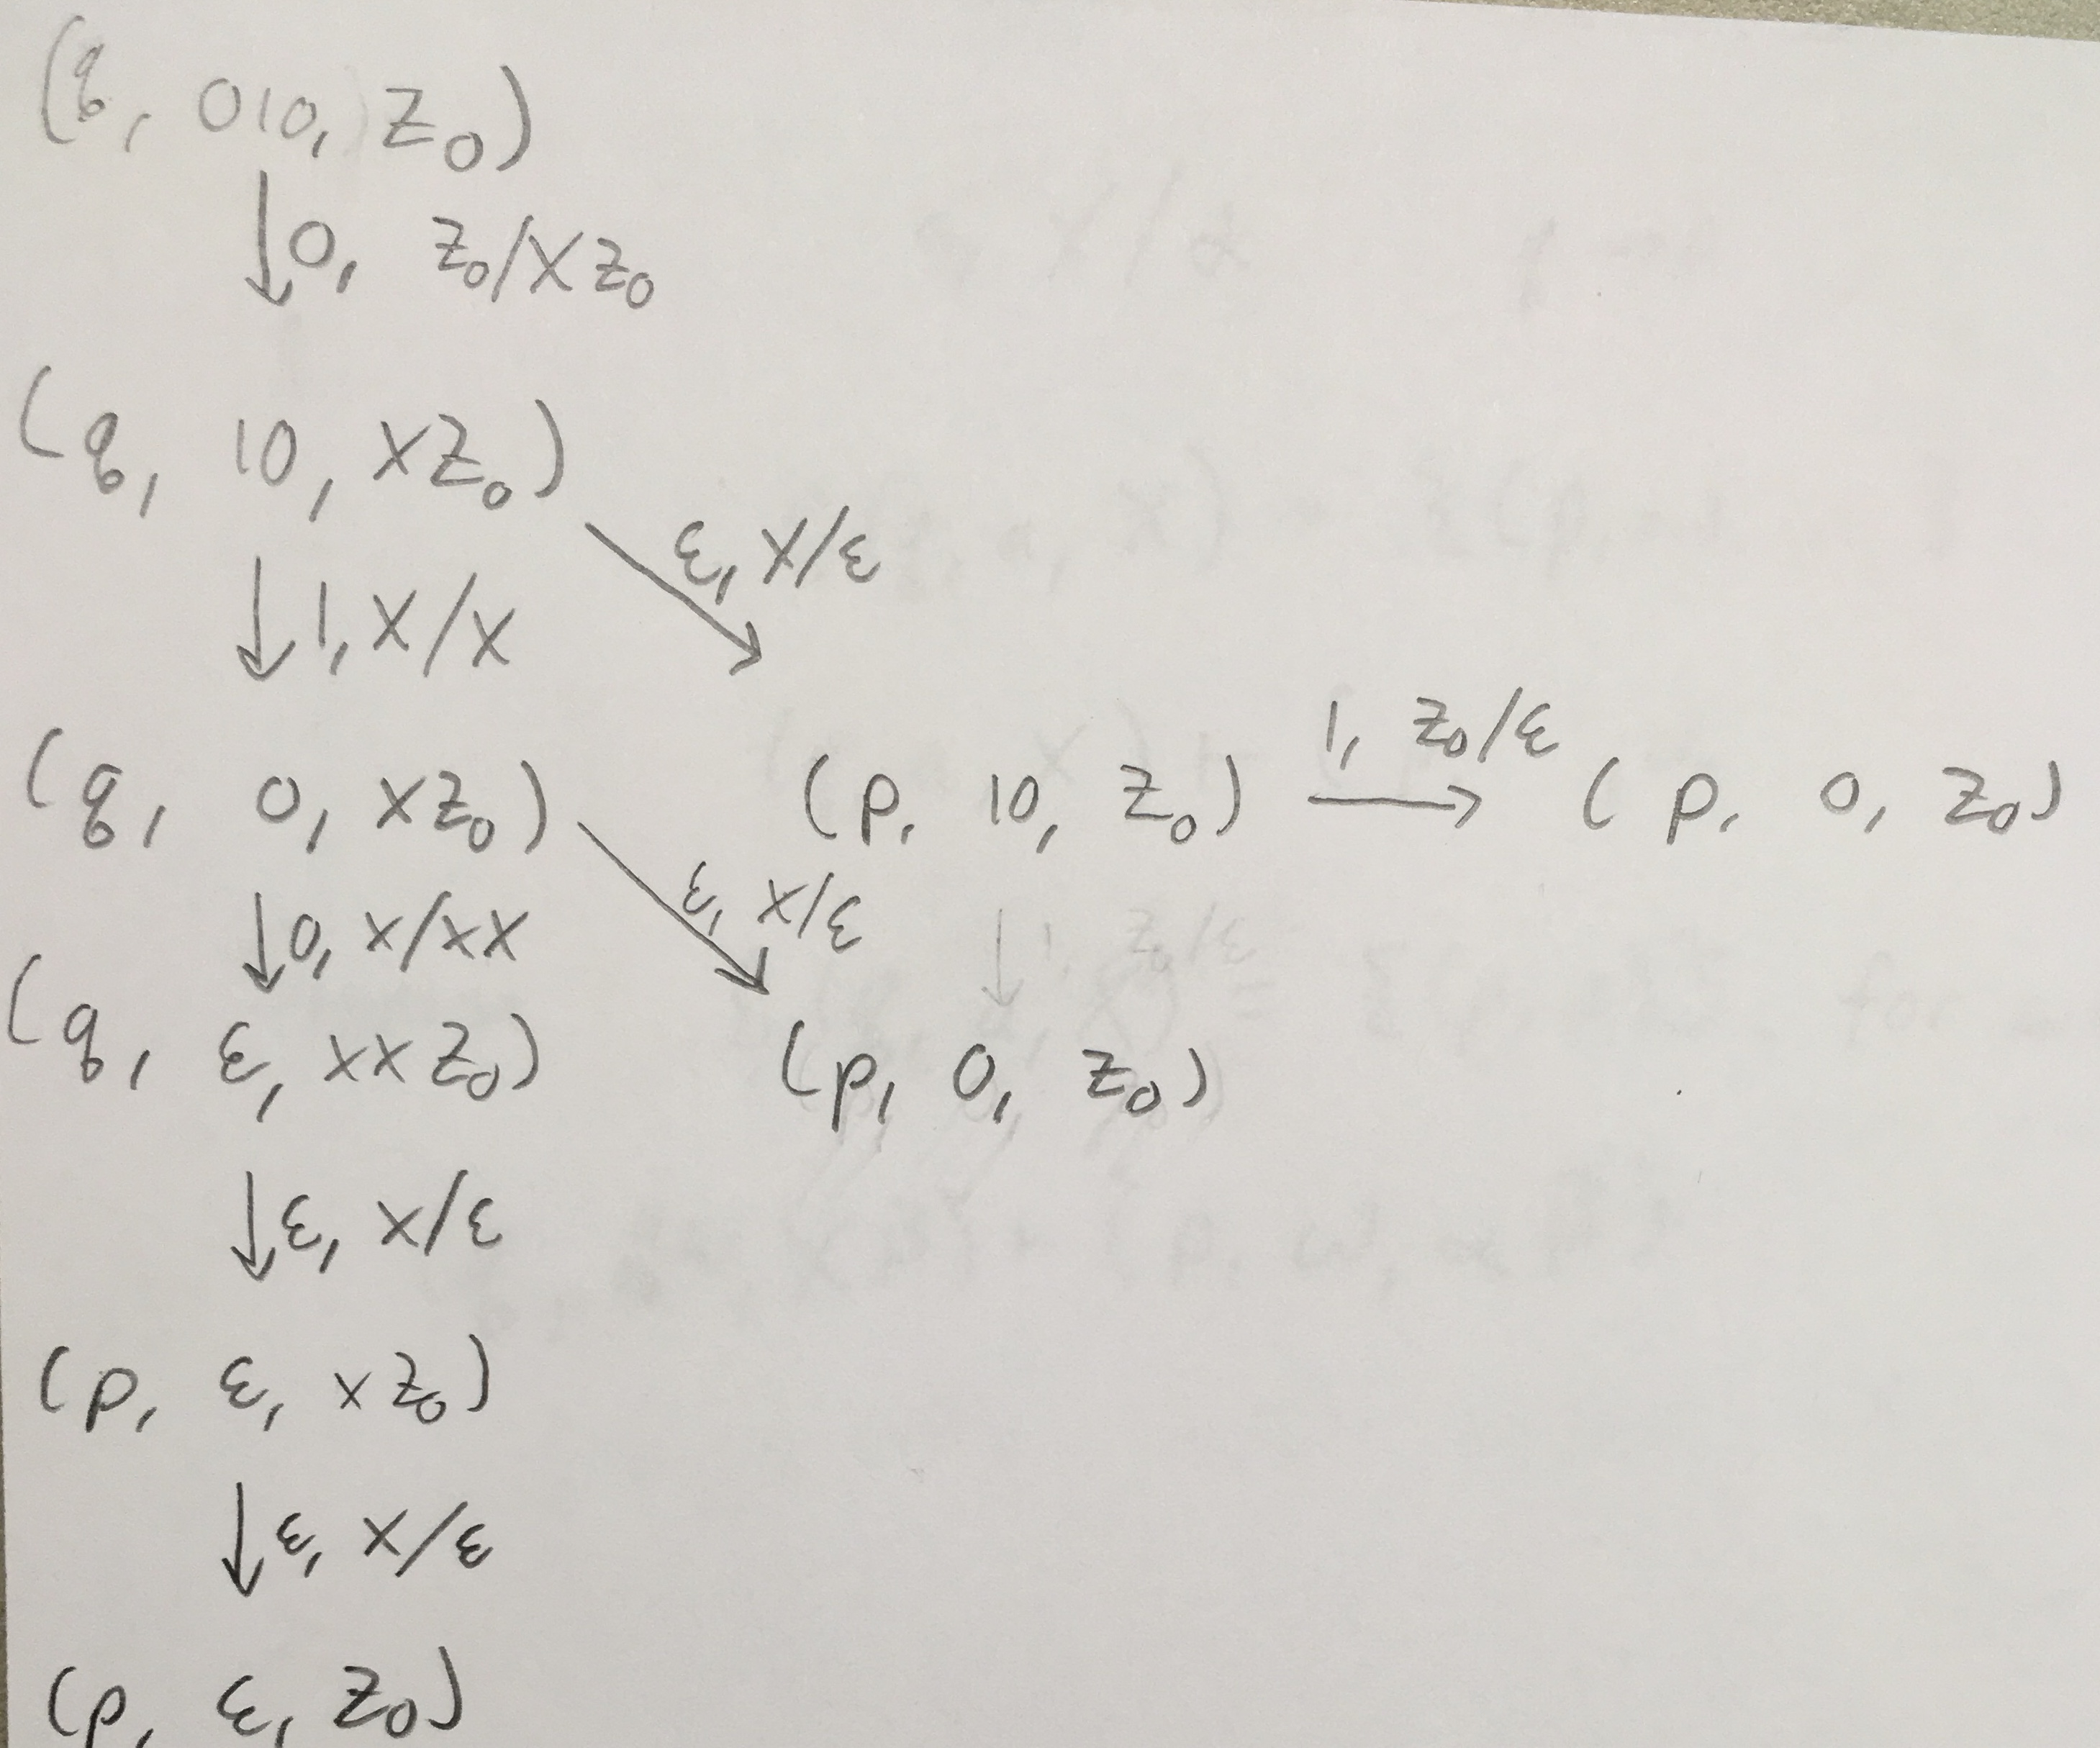
\includegraphics[width=\linewidth]{./figures/h7-3.jpg}
   	\end{subfigure}
\end{figure} 
\section{Problem 6.2.1}
Design a PDA to accept each of the following languages.  You may accept either by final state or by empty stack, whichever is more convenient.  
\subsection{a). $\{0^{n}1^{n} \mid n \geq 1\}$}
Let the PDA $\!P = (\{q_0, q_1, q_2\}, \{0,1\}, \{Z_0, X\}, \delta, q_0, \{q_2\})$. Then the rules for $\delta$ are: \\
\begin{enumerate}
\item $\delta(q_0, 0, Z_0) = \{(q_0, XZ_0)\}$
\item $\delta(q_0, 0, X) = \{(q_0, XX)\}$
\item $\delta(q_0, 1, X) = \{(q_1, \epsilon)\}$
\item $\delta(q_1, 1, X) = \{(q_1, \epsilon)\}$
\item $\delta(q_1, \epsilon, Z_0) = \{(q_2, Z_0)\}$
\end{enumerate}
\subsection{b). The set of all strings of 0's and 1's such that no prefix has more 1's than 0's.}
Let the PDA $\!P = (\{q_0, q_1\}, \{0,1\}, \{Z_0, X\}, \delta, q_0, \{q_1\})$. Then the rules for $\delta$ are: \\
\begin{enumerate}
\item $\delta(q_0, 1, Z_0) = \{(q_0, XZ_0)\}$
\item $\delta(q_0, 1, X) = \{(q_0, XX)\}$
\item $\delta(q_0, 0, X) = \{(q_0, \epsilon)\}$
\item $\delta(q_0, 0, Z_0) = \{(q_0, Z_0)\}$
\end{enumerate}
\newpage
\subsection{c). The set of all strings of 0's and 1's with an equal number of 0's and 1's.}
Let the PDA $\!P = (\{q_0, q_1, q_2\}, \{0,1\}, \{Z_0, X\}, \delta, \{q_0, 1_1\}, \{q_2\})$. Then the rules for $\delta$ are: \\
\begin{enumerate}
\item $\delta(q_0, 1, Z_0) = \{(q_0, XZ_0)\}$
\item $\delta(q_0, 1, X) = \{(q_0, XX)\}$
\item $\delta(q_0, 0, X) = \{(q_0, \epsilon)\}$
\item $\delta(q_0, \epsilon, Z_0) = \{(q_2, Z_0)\}$
\item $\delta(q_1, 0, Z_0) = \{(q_1, XZ_0)\}$
\item $\delta(q_1, 0, X) = \{(q_1, XX)\}$
\item $\delta(q_1, 1, X) = \{(q_1, \epsilon)\}$
\item $\delta(q_1, \epsilon, Z_0) = \{(q_2, Z_0)\}$
\end{enumerate}
\section{Problem 6.3.2}
Convert the grammar to a PDA that accepts the same language by empty stack \\
 \begin{table}[!htbp]
 \[\begin{array}{ccc} 
 S & \rightarrow & 0S1 \mid A \\
 A & \rightarrow & 1A0 \mid S \mid \epsilon \\
 \end{array}\]
 \end{table}
The rules for the transition function $\delta$ are: \\
\begin{enumerate}
\item $\delta(q, \epsilon, S) = \{(q, A), (q, 0S1)\}$
\item $\delta(q, \epsilon, A) = \{(q, \epsilon), (q, 1A0), (q, S)\}$
\item $\delta(q, 0, 0) = \{(q, \epsilon)\}$
\item $\delta(q, 1, 1) = \{(q, \epsilon)\}$
\end{enumerate}
\newpage
\section{Problem 6.4.1}
For each of the following PDA's, tell whether or not it is deterministic.  Either show that it meets the definition of a DPDA or find a rule or rules that violate it.
\subsection{The PDA of Example 6.2}
Because the PDA must choose when to move to the next state and process the other half of the string to verify a match, the PDA cannot be deterministic. If it were a DPDA, there would be no choice.
\subsection{The PDA of Exercise 6.1.1}

\subsection{The PDA of Exercise 6.3.3}
The PDA $\!P = (\{q, p\}, \{0,1\}, \{Z_0,X\}, \delta, q , Z_0)$, where  $\delta$ is defined to be:
\begin{enumerate}
\item $\delta(q, 1, Z_0) = \{(q, XZ_0)\}$.
\item $\delta(q, 1, X) = \{(q, XX)\}$.
\item $\delta(q, 0, X) = \{(p, X)\}$.
\item $\delta(q, \epsilon, X) = \{(q, \epsilon)\}$.
\item $\delta(p, 1, X) = \{(p, \epsilon)\}$.
\item $\delta(p, 0, Z_0) = \{(q, Z_0)\}$.
\end{enumerate}
\noindent\rule{2cm}{0.4pt} \\

\section{Problem 6.4.2}
Give deterministic pushdown automata to accept the following languages:
\subsection{a). $\{0^{n}1^{m} \mid n \leq m\}$}
\subsection{b). $\{0^{n}1^{m} \mid n \geq m\}$}
\subsection{c). $\{0^{n}1^{m}0^{n} \mid n$ and $m$ are arbitrary $\}$.}
$P = (\{q_0, q_1, q_2, q_3\}, \{0,1\}, \{Z_0, X\}, \delta, q_0, \{q_3\}$.
\begin{enumerate}
\item $\delta(q_0, 0, Z_0) = \{(q_0, XZ_0)\}$
\item $\delta(q_0, 0, X) = \{(q_0, XX)\}$
\item $\delta(q_0, \epsilon, Z_0) = \{(q_1, Z_0)\}$
\item $\delta(q_0, \epsilon, X) = \{(q_1, X)\}$
\item $\delta(q_1, 1, X) = \{(q_1, X)\}$
\item $\delta(q_1, 0, X) = \{(q_2, \epsilon)\}$
\item $\delta(q_1, \epsilon, Z_0) = \{(q_2, Z_0)\}$
\item $\delta(q_2, 0, X) = \{(q_2, \epsilon)\}$
\item $\delta(q_2, \epsilon, Z_0) = \{(q_3, Z_0)\}$
\end{enumerate}
\end{document}






































